% =====================================================================
% DIGEST VERSION -- results and figures only, minimal theory.
% Full record: paper/master/haatim_hsgs_master.tex (13 pp.)
% Submission version: paper/merged/haatim_hsgs_bounds_and_effective_rank.tex
%
% Every number here is copied from the master, where it carries a
% % SOURCE comment naming its store. The three experiment families are
% tagged [B3] [EXT] [TD] so no number is read against the wrong one:
%   [B3]  results/track_b/b3/           N in {8,16,32} x P in {10,30} x 6 SNR, 400 trials/pt
%   [EXT] trackB_hankel_emgs/results/   P=30 only, 7 SNR, 600/400/200 trials
%   [TD]  results/track_d/partB9/       N in {16,32,64}, P=20, adaptive order, 1 Cadzow sweep
% =====================================================================
\documentclass[11pt]{article}

\usepackage[a4paper,margin=2.3cm,top=2.0cm,bottom=2.0cm]{geometry}
\usepackage{amsmath,amssymb}
\usepackage{graphicx}
\usepackage{booktabs}
\usepackage{enumitem}
\usepackage{xcolor}
\usepackage[hidelinks]{hyperref}
\usepackage[font=small,labelfont=bf,skip=4pt]{caption}
\usepackage{titlesec}
\usepackage{float}
% Let figures sit near where they are written AND let text fill the page:
% without this, a digest of this shape leaves half-empty pages.
\renewcommand{\topfraction}{0.92}
\renewcommand{\bottomfraction}{0.75}
\renewcommand{\textfraction}{0.06}
\renewcommand{\floatpagefraction}{0.75}
\setcounter{topnumber}{3}
\setcounter{bottomnumber}{2}
\setcounter{totalnumber}{5}

\definecolor{ink}{HTML}{1a1a1a}
\definecolor{tag}{HTML}{6b6b6b}
\definecolor{rule}{HTML}{c9c9c9}
\color{ink}

\titleformat{\section}{\large\bfseries}{\thesection.}{0.6em}{}
\titlespacing*{\section}{0pt}{14pt}{6pt}
\setlist[itemize]{leftmargin=1.1em,itemsep=2pt,topsep=3pt}
\setlength{\parskip}{4pt}
\setlength{\parindent}{0pt}

% family tag, e.g. \famtag{B3}
\newcommand{\famtag}[1]{{\footnotesize\textcolor{tag}{[#1]}}}
\newcommand{\rmax}{r_{\max}}
\newcommand{\bG}{\mathbf{G}}
\newcommand{\bS}{\mathbf{S}}
\newcommand{\bB}{\mathbf{B}}
\newcommand{\bW}{\mathbf{W}}
\newcommand{\bZ}{\mathbf{Z}}

\begin{document}

\begin{center}
{\LARGE\bfseries Hankel-Structured Channel Estimation}\\[3pt]
{\LARGE\bfseries for Rydberg Atomic MIMO Receivers}\\[8pt]
{\large Results digest}\\[6pt]
{\normalsize Abdullah Haatim \quad$\cdot$\quad Department of Electrical and
Electronics Engineering}\\
{\normalsize BITS Pilani --- Pilani Campus}
\end{center}

\vspace{2pt}
\hrule height 0.6pt
\vspace{10pt}

{\small
Short version. All numbers are traceable; the full derivations, methodology and
provenance are in the master document. Three experiment families appear here
and are \emph{never} pooled --- each number is tagged \famtag{B3} \famtag{EXT} or
\famtag{TD} (\S\ref{sec:families}).
\par}

\vspace{6pt}

% =====================================================================
\section{The problem, in three sentences}
% =====================================================================

A Rydberg atomic receiver reads a radio field through an optical transition
whose response tracks field \emph{magnitude}. So the receiver measures
\begin{equation*}
\bZ = \bigl|\,\bG\bS + \bB + \bW\,\bigr|,
\end{equation*}
where $\bG$ is the $N\times K$ channel we want, $\bS$ the pilots, $\bB$ a known
reference field and $\bW$ noise --- \textbf{phase is lost, and the noise sits
inside the modulus}. Multi-user channel estimation is therefore a phase
retrieval problem, and the standard baseline is Gerchberg--Saxton with an EM
refinement (EM-GS).

% =====================================================================
\section{The idea, in one picture}
% =====================================================================

For a uniform linear array each channel column is a sum of $L$ complex
exponentials in the element index. Stack it into a Hankel matrix and that sum
becomes a rank-$L$ matrix:
\begin{equation*}
\mathcal{H}(\mathbf{g}) = \sum_{\ell=1}^{L}\alpha_\ell\,
\mathbf{v}_\ell\mathbf{w}_\ell^{\!\top}
\quad\Longrightarrow\quad
\operatorname{rank}\mathcal{H}(\mathbf{g}) \le L .
\end{equation*}
So \textbf{HS-GS} = EM-GS with a low-rank Hankel projection inserted after every
update. Two things make it non-trivial:

\begin{itemize}
\item \textbf{The prior has a capacity.} An $N$-element array can express at
most $\rmax(N)=\lceil N/2\rceil$ ranks. If $L\ge\rmax$ the constraint says
nothing. That is why the method's value depends on aperture.
\item \textbf{The order $\hat L$ must be chosen without an oracle.} It is
selected from held-out pilots. When the selector returns $\hat L\ge\rmax$ the
projection switches off --- the method \emph{abstains} rather than impose
structure it cannot support.
\end{itemize}

With the projection disabled, HS-GS reproduces EM-GS to $\max|\text{diff}|=0$.
The projection is provably the only difference between them.

\begin{figure}[!ht]
\centering
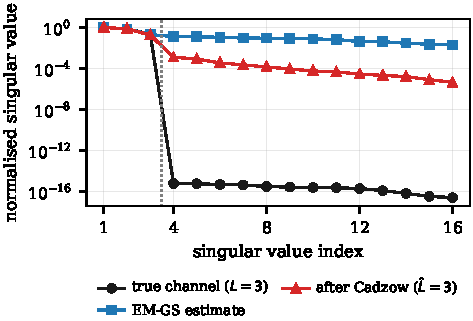
\includegraphics[width=0.60\textwidth]{fig/fig4_hankel_spectrum.pdf}
\caption{\textbf{Why the prior exists, and what the projection actually
achieves.} \famtag{EXT} Hankel singular values for one channel column
($N=32$, $L=3$). The true channel is exactly rank $L$
($\sigma_4/\sigma_1=5.7\times10^{-16}$). The EM-GS estimate is full numerical
rank ($0.130$) --- noise fills the spectrum. Four Cadzow sweeps restore the
cliff, but only to $1.2\times10^{-3}$: the structure is imposed
\emph{approximately}, which caps how much of the available gain the method can
capture. One illustrative realisation.}
\end{figure}

% =====================================================================
\section{Headline results}
% =====================================================================

Table~\ref{tab:head} is the whole story in one place. If you read nothing else,
read the first four rows: the method works, and \emph{how well} it works is
governed by array size, in a way the next section explains.

\begin{table}[!ht]
\centering
\small
\begin{tabular}{p{7.3cm}lc}
\toprule
\textbf{Result} & \textbf{Value} & \textbf{Family} \\
\midrule
Gain of HS-GS over EM-GS at $N=32$, $P=30$ & $+2.27$ to $+3.04$ dB & B3 \\
Aperture scaling, $N=8/16/32$ & $-0.19$ / $+0.78$ / $+2.85$ dB & B3 \\
Fraction of trials HS-GS wins, $N=8/16/32$ & $33.5$ / $74.0$ / $95.3\%$ & B3 \\
Constraint active, $N=8/16/32$ & $57.5$ / $92.7$ / $99.6\%$ & B3 \\
\addlinespace
EM-GS vs.\ Cram\'er--Rao bound, SNR $\ge5$ dB & within $0.051$ dB & B3 \\
Constrained bound below unconstrained one & $7.05$--$7.11$ dB & B3 \\
\addlinespace
Path-count decay, $L=2\to16$ & $+7.04\to-0.12$ dB & EXT \\
EM-GS is flat in both $N$ and $L$ & $0.012$ / $0.191$ dB & B3 / EXT \\
\addlinespace
Effective-rank zero crossing, $N=16/32/64$ & $0.588$ / $0.518$ / $0.544$ & TD \\
Prospective prediction error, gen.\ 1 / gen.\ 2 & $0.13$ / $0.315$ dB & TD \\
Gain invariance in user count $K$, SNR $\ge5$ dB & $0.095$ dB spread & TD \\
\bottomrule
\end{tabular}
\caption{The numbers worth remembering. The two flatness figures are the
control: EM-GS ignores structure, so it should not move when structure changes
--- and it does not.}
\label{tab:head}
\end{table}

\begin{figure}[!ht]
\centering
\begin{minipage}[t]{0.49\textwidth}
\centering
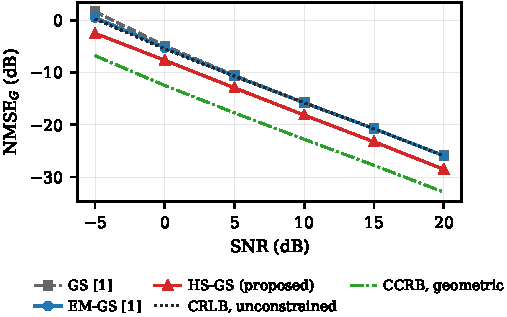
\includegraphics[width=\textwidth]{fig/fig1_nmse_vs_snr.pdf}
\end{minipage}\hfill
\begin{minipage}[t]{0.49\textwidth}
\centering
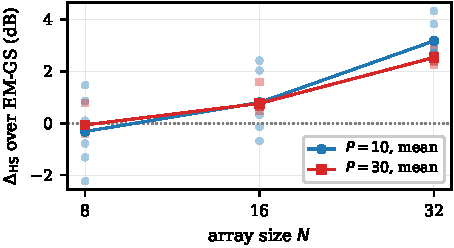
\includegraphics[width=\textwidth]{fig/fig2_gain_vs_N.pdf}
\end{minipage}
\caption{\textbf{Left: the main result.} \famtag{B3} NMSE vs.\ SNR at $N=32$,
$K=3$, $P=30$, 400 paired trials per point. HS-GS beats EM-GS by $2.27$--$3.04$
dB across the sweep. EM-GS itself tracks the unconstrained CRLB to within
$0.051$ dB above 5 dB, which is what makes the benchmark meaningful rather than
vacuous. \textbf{Right: the gain depends on aperture.} \famtag{B3} It is
\emph{negative} at $N=8$, where capacity $\rmax=4$ is smaller than the typical
path count.}
\end{figure}

% =====================================================================
\section{The three findings that matter}
% =====================================================================

\textbf{1. The gain is controlled by how much of the prior's capacity the
channel uses --- not by array size or path count on their own.}
A controlled sweep confirms the mechanism directly: hold everything fixed and
vary only $L$, and the gain decays monotonically from $+7.04$ dB at $L=2$ to
$-0.12$ dB at $L=16=\rmax$ \famtag{EXT}. EM-GS does not move ($0.191$ dB across the
whole sweep), which is exactly what an estimator that ignores structure should
do.

\textbf{2. Raw path count is the wrong coordinate; effective rank is the right
one.} Replacing $L$ by the effective rank of the Hankel matrix
($r_{\mathrm{eff}}=\exp(-\sum p_i\ln p_i)$, normalised by capacity) collapses
three different array sizes onto one curve, crossing zero at
$0.588/0.518/0.544$ for $N=16/32/64$ \famtag{TD}. The \emph{location} of the
boundary is array-invariant to within $0.07$.

\textbf{3. The coordinate predicts, not just describes.} Two channel generators
never used to build the relation were run, with predictions committed to
version control \emph{before} measurement and with no refitting. Errors:
$0.13$ dB and $0.315$ dB \famtag{TD}.

\begin{figure}[!ht]
\centering
\begin{minipage}[t]{0.49\textwidth}
\centering
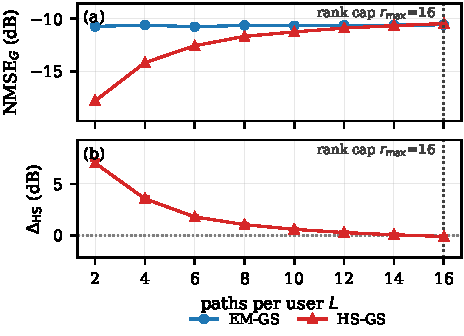
\includegraphics[width=\textwidth]{fig/fig3_pathcount.pdf}
\end{minipage}\hfill
\begin{minipage}[t]{0.49\textwidth}
\centering
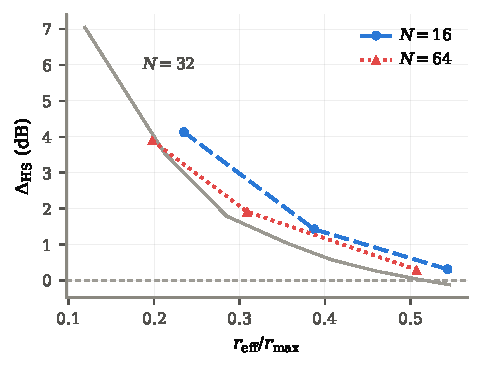
\includegraphics[width=\textwidth]{fig/fig7_boundary_invariance.pdf}
\end{minipage}
\caption{\textbf{Left: the controlled experiment.} \famtag{EXT} Vary only the path
count $L$. The gain decays to zero exactly as $L$ approaches capacity
$\rmax=16$; EM-GS stays flat. The hypothesis was recorded before the run.
\textbf{Right: the collapse.} \famtag{TD} Plotted against effective rank over
capacity, three array sizes land on one curve and cross zero at nearly the same
place.}
\end{figure}

\begin{figure}[!ht]
\centering
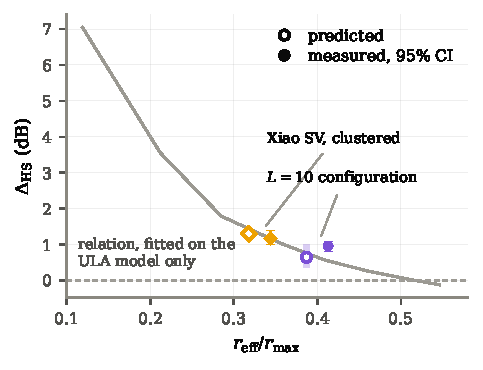
\includegraphics[width=0.60\textwidth]{fig/fig8_cross_generator.pdf}
\caption{\textbf{Predictions registered before measurement.} \famtag{TD} Hollow
markers are what the relation predicted; filled markers with bars are what was
measured, with 95\% confidence intervals. The relation was fitted on the ULA
model only and was \emph{not} refitted for either generator. The prediction
rule is a piecewise-linear interpolation on a fixed 8-point table --- no
regression, no spline, so it can be re-executed exactly.}
\end{figure}

% =====================================================================
\section{What does not work}
% =====================================================================

Stated plainly, because these bound how far the result travels.

\begin{itemize}
\item \textbf{$N=8$ is a mixed result, not a small positive one.} The gain is
$+1.47$ dB at $-5$ dB SNR but falls to $-2.23$ dB at high SNR, and the
projection is inactive in $42.5\%$ of trials \famtag{B3}. Truncation bias does not
shrink with noise, so as SNR rises the trade stops paying and then reverses.
The sign of any single scalar summary at $N=8$ depends on the pooling.
\item \textbf{The collapse is imperfect.} The \emph{location} of the boundary is
array-invariant; the gain \emph{magnitude} is not. A one-signed residual of mean
$0.493$ dB (max $0.901$) between $N=16$ and $N=64$ is unexplained \famtag{TD}.
\item \textbf{A pre-registered criterion narrowly failed.} The $K$-invariance
test misses its own falsifier by $0.006$ dB when pooled over all SNR
(it passes comfortably at SNR $\ge5$ dB) \famtag{TD}. Reported, not dropped.
\item \textbf{The second prediction is an order of magnitude worse than the
first} ($0.315$ vs.\ $0.13$ dB), though still inside its stated interval.
\item \textbf{The bounds do not formally govern the estimators plotted against
them.} CRLB and CCRB constrain \emph{unbiased} estimators; every estimator here
is biased. They are informative benchmarks, not laws these curves must obey.
\item \textbf{Simulation only}, geometric ULA channels only, and order selection
costs $57.7$--$85.5\%$ of runtime with no attempt yet to reduce it.
\end{itemize}

% =====================================================================
\section{The three experiment families}\label{sec:families}
% =====================================================================

These are \textbf{different experiments}. Numbers from one are not comparable
to numbers from another as measurements of the same thing.

\begin{table}[!ht]
\centering
\small
\begin{tabular}{llp{7.4cm}}
\toprule
\textbf{Tag} & \textbf{Store} & \textbf{Configuration} \\
\midrule
B3 & \texttt{results/track\_b/b3/} &
$N\in\{8,16,32\}$, $P\in\{10,30\}$, 6 SNR points, 400 trials/point,
4 Cadzow sweeps. The principal experiment. \\
\addlinespace
EXT & \texttt{trackB\_hankel\_emgs/} &
$P=30$ only, 7 SNR points, 600/400/200 trials. A separate diagnostic run. \\
\addlinespace
TD & \texttt{results/track\_d/partB9/} &
$N\in\{16,32,64\}$, $P=20$, adaptive order, \emph{1} Cadzow sweep. One sweep and
four sweeps define different operators. \\
\bottomrule
\end{tabular}
\end{table}

B3 and EXT both measure aperture gain and \emph{disagree}
($-0.19/+0.78/+2.85$ vs.\ $+0.03/+0.81/+2.45$ dB) because they are different
experiments. Both are correct for their own configuration; neither should be
quoted for the other.

\vspace{10pt}
\hrule height 0.4pt
\vspace{6pt}

{\small\textcolor{tag}{Full document with derivations, algorithms, methodology
and complete limitations:\\
\texttt{paper/master/haatim\_hsgs\_master.pdf} (13 pp.). Verification of every
number against its store:\\
\texttt{paper/master/MASTER\_PAPER\_AUDIT.md}. No simulation was rerun to
produce this digest.}\par}

\end{document}
